\documentclass{article}

\usepackage{geometry}
\usepackage{amsmath}
\usepackage{graphicx, eso-pic}
\usepackage{listings}
\usepackage{hyperref}
\usepackage{multicol}
\usepackage{fancyhdr}
\usepackage{tikz}
\pagestyle{fancy}
\fancyhf{}
\hypersetup{ colorlinks=true, linkcolor=black, filecolor=magenta, urlcolor=cyan}
\geometry{ a4paper, total={170mm,257mm}, top=40mm, right=20mm, bottom=20mm, left=20mm}
\setlength{\parindent}{0pt}
\setlength{\parskip}{0.3em}
\renewcommand{\headrulewidth}{0pt}
\AddToShipoutPictureBG{%
  \AtPageUpperLeft{%
    \raisebox{-\height}{
\includegraphics[width=\paperwidth, height=30mm]{../headerarkav.png}}
  }
}
\rfoot{\thepage}
\lfoot{Penyisihan Competitive Programming - Arkavidia 7.0}
\lstset{
    basicstyle=\ttfamily\small,
    columns=fixed,
    extendedchars=true,
    breaklines=true,
    tabsize=2,
    prebreak=\raisebox{0ex}[0ex][0ex]{\ensuremath{\hookleftarrow}},
    frame=none,
    showtabs=false,
    showspaces=false,
    showstringspaces=false,
    prebreak={},
    keywordstyle=\color[rgb]{0.627,0.126,0.941},
    commentstyle=\color[rgb]{0.133,0.545,0.133},
    stringstyle=\color[rgb]{01,0,0},
    captionpos=t,
    escapeinside={(\%}{\%)}
}

\begin{document}

\begin{center}
    \section*{D - DVD} % ganti judul soal

    \begin{tabular}{ | c c | }
        \hline
        Batas Waktu  & 2s \\    % jangan lupa ganti time limit
        Batas Memori & 256MB \\  % jangan lupa ganti memory limit
        \hline
    \end{tabular}
\end{center}

\subsection*{Deskripsi}

Terdapat matriks berukuran $N \times M$ yang pada awalnya berisi $0$. Terdapat sebuah sinar datang dari koordinat $(0, 0)$ dengan sudut $45^{\circ}$ ke arah kanan bawah. Setiap kotak yang dilewati sinar ini akan berubah nilainya menjadi warna sinar tersebut. Warna sinar ditandai dengan angka $1$ sampai $9$, dimulai dari warna $1$. Apabila sinar dipantulkan, warna sinar akan berubah menjadi warna selanjutnya (dari $1$ menjadi $2$, dari $2$ menjadi $3$, dan seterusnya). Jika sebuah kotak dilalui dua kali, warna terakhir yang akan digunakan. Pantulan sinar akan terhenti bila sinar mengenai salah satu sudut. Contoh untuk $N$ = 4 dan $M$ = 6, hasil pantulannya adalah:

\begin{center}
	\begin{tikzpicture}
	%\draw (0,0) -- (4,4);
	\draw [color=blue, thick, ->] (0,4) -- (4,0);
	\draw [color=red, thick, ->] (4,0) -- (6,2);
	\draw [color=green, thick, ->] (6,2) -- (4,4);
	\draw [color=yellow, thick, ->] (4,4) -- (0,0);
	\draw[step=1cm,gray,very thin] (0,0) grid (6,4);
	\node[inner sep=0pt] (dvd) at (0,4)
    		{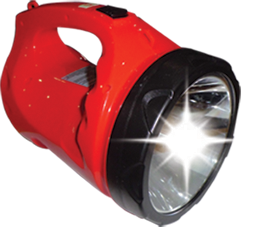
\includegraphics[width=.05\textwidth]{senter.png}};
	\node at (+0.5,+3.5) {1};
	\node at (+1.5,+2.5) {1};
	\node at (+2.5,+1.5) {1};
	\node at (+3.5,+0.5) {1};
	\node at (+4.5,+0.5) {2};
	\node at (+5.5,+1.5) {2};
	\node at (+5.5,+2.5) {3};
	\node at (+4.5,+3.5) {3};
	\node at (+3.5,+3.5) {4};
	\node at (+2.5,+2.5) {4};
	\node at (+1.5,+1.5) {4};
	\node at (+0.5,+0.5) {4};
	\end{tikzpicture}
\end{center}

Diberikan $Q$ query, yang masing-masing berisi empat bilangan $N, M, X, Y$. Untuk setiap query, Anda diminta untuk mengeluarkan sebuah bilangan, berupa nilai bilangan pada koordinat $(X, Y)$ di matriks yang berukuran $N \times M$.

\subsection*{Format Masukan}
Baris pertama berisi sebuah bilangan bulat $Q$ $(1 \leq Q \leq 10^3)$, menyatakan banyaknya query.

$Q$ baris berikutnya berisi empat buah bilangan bulat $N, M, X, Y$ $(1 \leq N, M \leq 10^6, 1 \leq X \leq N, 1 \leq Y \leq M)$, masing-masing menyatakan ukuran baris matriks, ukuran kolom matriks, serta warna koordinat baris dan kolom yang dicari.

\subsection*{Format Keluaran}
$Q$ baris yang berisi sebuah bilangan bulat yang merupakan warna kotak berkoordinat ($X, Y$)

\begin{multicols}{2}
\subsection*{Contoh Masukan}
\begin{lstlisting}
2
4 6 2 1
3 4 2 3
\end{lstlisting}
\columnbreak
\subsection*{Contoh Keluaran}
\begin{lstlisting}
4
2
\end{lstlisting}
\vfill
\null
\end{multicols}

\subsection*{Penjelasan}
Hasil pantulan untuk query pertama terletak pada deskripsi soal, sehingga didapat bahwa bilangan yang terdapat pada koordinat $(2, 1)$ adalah 4.

\pagebreak

\end{document}